\chapter{The Standard Model}

\subsection{Overview}

The Standard Model is another name for the theory of the internal symmetry group $SU(3)_C \otimes SU(2)_L \otimes U(1)_Y$ \todo{CHECK}.
This quantum field theory is the culmination of years of work in both theoretical and particle physics.  \todo{cite}

\todo{CITE THIS PICTURE}
\begin{figure}
\caption{The interactions of the Standard Model}
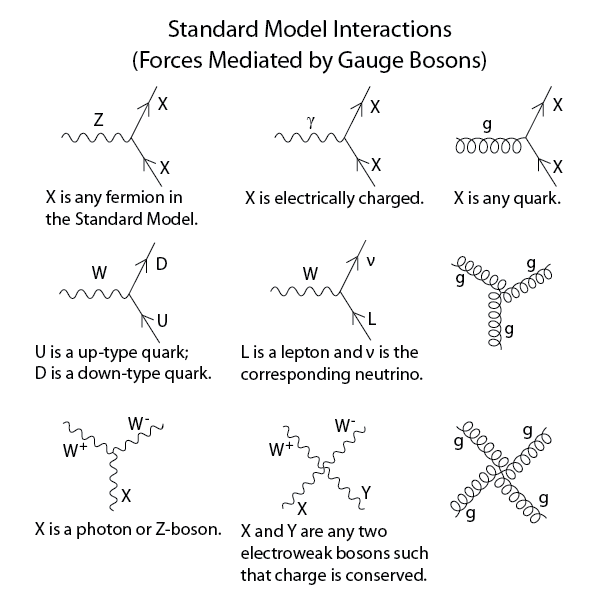
\includegraphics[width=\linewidth]{Standard_Model_Feynman_Diagram_Vertices}
\end{figure}

\subsection{Field Content}

The SM field content is
\begin{equation}
\begin{aligned}
\text{Fermions } Q_L(3,2)_{+1/3}, \xspace  U_R(3,1)_{+4/3},\xspace  D_R(3,1)_{-2/3} ,\xspace  L_L(1,2)_{-1} ,\xspace  E_R(1,1)_{-2}\\
\text{Scalar (Higgs) } \xspace \phi(1,2)_{+1} \\
\text{Vector Fields } \xspace G^\mu(8,1)_0 \xspace W^\mu(1,3)_0  \xspace B^\mu(1,1)_0
\end{aligned}
\end{equation}
where the $(A, B)_Y$ notation represents the irreducible representation under $SU(3)$ and $SU(2)$, with $Y$ being the electroweak hypercharge.
Each of these fields has an additional index, representing the three generation of fermions.

We observed that $Q_L, U_R,$ and $D_R$ are triplets under $SU(3)_C$; these are the \textit{quark} fields.
The ``color'' group, $SU(3)_C$ is mediated by the ``gluon'' field $G^\mu(8,1)_0$, which has 8 degrees of freedom; we say there are 8 gluons.
The fermion fields $L_L(1,2)_{-1}$ and $  E_R(1,1)_{-2} $ are singlets under $SU(3)_C$; we call them \textit{leptons}.

Next, we note the ``left-handed'' (``right-handed'') fermion fields, denoted by $L$ ($R$) subscript,
The left-handed fields form doublets under $SU(2)_L$.
These are mediated by the three degrees of freedom of the  ``W'' fields $W^\mu(1,3)_0$.
These fields only act on the left-handed particles of the Standard Model.
This is the reflection of the ``chirality'' of the Standard Model; the left-handed and right-handed particles are treated differently by the electroweak forces.
The right-handed fields, $U_R, D_R$, and $E_R$, are singlets under $SU(2)_L$.

The $U(1)_Y$ symmetry is associated to the $B^\mu(1,1)_0$ boson with one degree of freedom.
The charge $Y$ is known as the electroweak hypercharge.

\subsection{$\Lagr_{kin}$}

For each of the vector boson fields, we have the follow field strengths :

\begin{equation}
\begin{aligned}
G^{\mu\nu}_a = \dmuup G^\nu_a + \partial^\nu G^\mu_a - g_s f_{abc} G^\mu_b G^\nu_c \\
W^{\mu\nu}_a = \dmuup W^\nu_a + \partial^\nu W^\mu_a - g \epsilon_{abc} W_b^\mu W_c^\nu \\
B^{\mu\nu}   = \dmuup B^\nu   + \partial^\nu B^\mu
\end{aligned}
\end{equation}

where $g$ and $g_s$ are the electroweak and strong coupling constant.

We can write the covariant derivative for the Standard Model as
\begin{equation}
\Dmuup = \dmuup + ig_s G^\mu_a L_a + i g W^\mu_a T_a + i g' Y B^\mu
\end{equation}
where $L_a$ and $T_a$ are the generators of $SU(3)_C $ and $SU(2)_L$ respectively for each of the representations.
Explicitly, for the $SU(3)_C$ triplets, $L_a = \frac{1}{2} \lambda_a$ and for the $SU(3)_C$ singlets, $L_a = 0$. \todo{GELLMANN and Pauli matrices}.
For $SU(2)_L$ doublets, $T_a = \frac{1}{2} \sigma_a $ and for $SU(2)_L$ singlets, $T_a = 0$.

The combination of these terms allows us to write the kinetic terms of the Lagrangian as
\begin{equation}
\begin{aligned}
\Lagr_{kin} = G^{\mu\nu} G_{\mu\nu} + W^{\mu\nu} W_{\mu\nu} + B^{\mu\nu} B_{\mu\nu}\\
 + \Dmuup Q_L \Dmu Q_L + \Dmuup U_R \Dmu U_R +  \Dmuup D_R \Dmu D_R + \Dmuup L_L \Dmu L_LL + \Dmuup E_R \Dmu E_R
\end{aligned}
\end{equation}

\subsection{$\Lagr_{\psi}$ }

We cannot write down any mass terms for fermions in the Standard Model.
Dirac mass terms are forbidden since they are all assigned to ``chiral'' representations of the gauge symmetry.
Majorana mass terms are disallowed since there are no fields with $Y \slashed{=} 0$.

\subsection{$\Lagr_{Yuk}$ }

We write the Yukawa portion of the Standard Model Lagrangian

\begin{equation}
\Lagr_{Yuk} = Y_{ij}\bar{L_{Li} E_{Rj}} \phi + h.c.
\end{equation}

The Yukawa matrix $Y$ is a general complex 3 $\times$ 3 matrix of dimensionless couplings which can be diagonalized, leading to a diagonal matrix with only three real parameters $(y_e , y_\mu , y_\tau)$.
This reflects the fact that for the electron, muon, and tau lepton, the interaction basis is the same as the mass basis; this is the same as saying an electron has a well-defined mass.

\section{$\Lagr_\phi$, Electroweak Symmetry breaking and the Higgs Boson}

Let us now recall that local gauge invariance means that the vector fields in this theory are \textit{massless}.
N\"aively, it seems this combined with the chirality of the Standard Model, that \textit{none} of the fields have masses.
The solution to this seeming conundrum is of course the well-known ``Higgs'' mechanism, described in Sec. \ref{subsec:symmetry_breaking}.

In the Standard Model, the Higgs potential is given by
\begin{equation} \label{eq:higgs_potential}
\Lagr_\phi = -\mu^2 \phi^\dagger \phi - \lambda (\phi^\dagger \phi)^2.
\end{equation}

Since $\lambda$ is dimensionless and real, to have a potential bounded from below, we require $\lambda > 0$.
To break the gauge symmetry, we require $\mu^2 < 0$, leading again to the sombrero potential \ref{fig:sombrero}.
We define
\begin{equation}
v^2 = - \frac{\mu^2}{\lambda}.
\end{equation}

This allows us to write \ref{eq:higgs_potential} as
\begin{equation} \label{eq:higgs_potential_rewritten}
\Lagr_\phi = - \lambda (\phi^\dagger \phi - \frac{v^2}{2})^2
\end{equation}
after dropping the constant term.

This means the $\phi$ field acquires a VEV $|<\phi>| = v/\sqrt{2}$.
Choosing the convenient gauge
\begin{equation}
\phi = \begin{pmatrix} 0 \\ v/\sqrt{2} \end{pmatrix},
\end{equation}

The VEV breaks the $SU(2)_L \otimes U(1)_Y$ symmetry to a $U(1)_{EM}$ subgroup.
We can identify the unbroken generator of this $U(1)_{EM}$ subgroup as $Q_{EM} = T_3 + Y/2$, since this vanishes in the down component
\begin{equation}
Q_{\gamma} \phi = (T_3 + Y/2) \phi = (\frac{1}{2} \sigmathree + \frac{1}{2} I ) \begin{pmatrix} 0 \\ v/\sqrt{2} \end{pmatrix}.
\end{equation}
Here we see the indicative $\gamma$ for the photon, as this unbroken $U(1)_{EM}$ symmetry is of course the symmetry associated to the electromagnetic force mediated by the gauge boson known as the photon.

There are three broken generators : $T_1, T_2, T_3 - Y/2$.
These are each associated to one of the massive gauge bosons induced by the symmetry breaking.
Choosing a gauge which rotates away the ``eaten'' Goldstone boson degrees of freedom, we can write the Higgs field as
\begin{equation}
\label{eq:higgs_field}
\phi = \frac{1}{\sqrt{2}}\begin{pmatrix} 0 \\ v + h(x) \end{pmatrix}.
\end{equation}

\section{Particle Spectrum : Standard Model Lagrangian after Electroweak Symmetry Breaking}

We can now return to the Standard Model Lagrangian and use the equation for the Higgs field after EWSB \ref{eq:higgs_field}.
This will show us the ``physical'' particle content of the Standard Model.

\subsection{Particle content associated to $\Lagr_\phi$}

Setting $phi$ as in Eq.\ref{eq:higgs_field}, we quickly see that we can rewrite Eq.\ref{eq:higgs_potential_rewritten} as
\todo{ CHECK FACTORS OF TWO}
\begin{equation}
\Lagr_\phi = - \lambda (\phi^\dagger \phi - \frac{v^2}{2})^2  = - \lambda ( \frac{1}{2} (v + h(x))^2 - \frac{v^2}{2})^2 = - \lambda ( h(x)^2 + vh(x))^2 = -\lambda ( h(x)^4 + v h(x)^3 + \frac{v^2}{2} h(x)^2 ).
\end{equation}

Interpreting the Higgs field squared term as the mass term of the Higgs boson, we see that $m_H = \sqrt{2 \lambda} v$.

\subsection{Particle content associated to $\Lagr_{kin}$}

Again using Eq.\ref{eq:higgs_field} and $\Dmuup = \dmuup + ig_s G^\mu_a L_a + i g W^\mu_a T_a + i g' Y B^\mu $, we can see how the mass terms associated to the three massive gauge bosons, and also see how the photon stays massless.
The mass terms for the gauge boson fields come from the kinetic term of the Higgs field :
\begin{equation}
\begin{aligned}
\Lagr_{M_V} = \Dmuup \phi \Dmu \phi = (i g W^\mu_a T_a + i g' Y B^\mu ) \frac{1}{\sqrt{2}}\begin{pmatrix} 0 \\ v \end{pmatrix} (i g W_{\mu,a} T_a + i g' Y B_\mu ) \frac{1}{\sqrt{2}}\begin{pmatrix} 0 \\ v \end{pmatrix} = \\
\frac{1}{8} |\begin{pmatrix} gW_3 + g'B & g(W_1 - iW_2) \\ g(W_1 + iW_2) & -gW_3 + g'B \end{pmatrix}  \begin{pmatrix} 0 \\ v \end{pmatrix} |^2
\end{aligned}
\end{equation}
where we have noted that $\dmu$ and $L_a$ both disappear when acting on $\phi$.
Defining the \textit{Weinberg} angle $\tan(\theta_W) = g'/g$ and the following physical fields :
\begin{equation}
\begin{aligned}
W^{\pm} = \frac{1}{\sqrt{2}}(W_1 \mp iW_2) \\
Z^0 = \cos \theta_W W_3 - \sin\theta_W B \\
A^0 = \sin \theta_W W_3 + \cos\theta_W B
\end{aligned}
\end{equation}
we see that we can write the piece of the Lagrangian associated to the vector boson masses as
\begin{equation}
\Lagr_{M_V} = \frac{1}{4} g^2 v^2 W^+ W^- + \frac{1}{8} (g^2 + g'^2)v^2 Z^0 Z^0 .
\end{equation}
and we have the following values of the masses for the vector bosons :
\begin{equation}
\begin{aligned}
m_W^2 = \frac{1}{4} g^2 v^2 \\
m_Z^2 = \frac{1}{4} (g^2 + g'^2) v^2 \\
m_A^2 = 0
\end{aligned}
\end{equation}

\section{Deficiencies of the Standard Model}

By using the asterisk to start a new section, I keep the section from appearing in the table of contents.
If you want your sections to be numbered and to appear in the table of contents, remove the asterisk.
